\documentclass[dvipdfmx]{jsarticle}
\usepackage[dvipdfmx]{graphicx}
\usepackage{amsmath, amssymb}
\usepackage{mathtools}
\usepackage{here}


\begin{document}

\section*{3.2 活性化関数}
式\ref{step}で表される活性化関数は,閾値を境にして出力が切り替わり,「ステップ関数」や「階段関数」と呼ばれる.よって,パーセプトロンは活性化関数にステップ関数を利用していると言える.この節では,ニューラルネットワークで用いられるいくつかの活性化関数を紹介する.
\begin{equation}\label{step}
    f(x)=
    \begin{dcases}
      0 & (x \leqq 0) \\
      1 & (x > 0)
    \end{dcases}
  \end{equation}


\section*{3.2.1 シグモイド関数}
ニューラルネットワークでよく用いられる活性化関数のひとつに,式\ref{sigmoid}で表される\textbf{シグモイド関数}(sigmoid function)がある.ニューラルネットワークでは,活性化関数にシグモイド関数を用いて信号の変換を行い,その変換された信号が次のニューロンに伝えられる.
前章で学んだパーセプトロンとニューラルネットワークの主な相違点は,この活性化関数だけである.その他,ニューロンが多層につながる構造や,信号の伝達方法は基本的にパーセプトロンと同じである.
\begin{equation}\label{sigmoid}
h(x)=\frac{1}{1 + \exp(-x)}
\end{equation}


\section*{3.2.5 シグモイド関数とステップ関数の比較}
\begin{figure}[H]\label{step_sigmoid}
\begin{center}
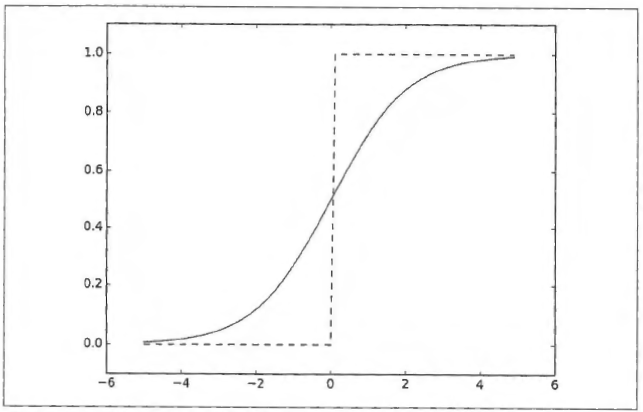
\includegraphics[width=0.8\linewidth]{"./spring_lec/dp_active_function.png"}
\end{center}
\caption{ステップ関数とシグモイド関数(破線はステップ関数)}
\end{figure}
シグモイド関数とステップ関数を図\ref{step_sigmoid}に示す.図\ref{step_sigmoid}を見ると,異なっている点として「滑らかさ」の違いが挙げられる.シグモイド関数は滑らかな曲線で,入力に対して連続的に実数を出力する.一方,ステップ関数は0を境に急に出力を変え,0か1のどちらかの値しか返さない.このシグモイド関数の滑らかさが,ニューラルネットワークにおいて重要な意味を持つ.

続いて,2つの関数の共通する性質について述べる.2つの関数は,滑らかさという点で異なるが,入力が小さいときに出力は0に近く(0であり),入力が大きくなるに従い出力が1に近づく(1になる)という点で,似た構造をしているということが分かる.つまり,ステップ関数とシグモイド関数は,入力信号が重要な情報であれば大きな値を出力し,入力信号が重要でなければ小さな値を出力するのである.そして,すべての入力信号に対し,出力信号の値を0から1の間に制限しているのも両者の共通点である.
\end{document}